\chapter{Interface Água/Metal \label{cap:equilibrio}}

%Nesse capítulo apresentaremos com mais detalhes os cálculos da interface água/Pd, bem como os resultados obtidos a partir das escolhas de cada etapa, tais como  a base, o pseudopotencial e o funcional de troca e correlação. Na Seção \ref{bulk} serão apresentados os detalhes computacionais utilizados nos cálculos de bulk e de slab do Pd, bem como os resultados obtidos. Uma vez caracterizadas as propriedades do metal, serão realizadas simulações com a água adsorvida no metal, com a estrutura de monômero e camada, Seção \ref{agua}. Aqui mostraremos a influência da escolha do funcional, quantidade de pontos k, tamanho da célula unitária e erro de superposição de base no valor da energia de adsorção. Por fim, na Seção \ref{sec:smeagol} construiremos a geometria do sistema para realizar os cálculos com um potencial aplicado via Funções de Green Fora do Equilíbrio (NEGF) e mostraremos os resultados preliminares.
Nesse capítulo caracterizamos a interface água/metal através das propriedades estruturais, energéticas e vibracionais de estruturas de água adsorvida no Pd(111). Para isso, estudamos a adsorção de monômero e de camada de água sobre a superfície metálica, cujos resultados estão descritos nas Seções \ref{sec:agua} e \ref{sec:re-la}, respectivamente. No primeiro sistema, a única interação existente é a do tipo água/metal, ao passo que na camada de água temos também ligações de hidrogênio entre as moléculas de água. Essas últimas podem ser impactadas pela presença de uma superfície metálica. Em particular, a intensidade dessas forças são semelhantes, de modo que, a estabilidade do sistema é definida pela competição entre os dois tipos de interação. Portanto, caracterizar as geometrias, energias e os modos vibracionais de uma estrutura adsorvida em um metal fornece detalhes sobre as interações envolvidas e sobre qual força é dominante. 

%As rotinas computacionais foram executadas pelo Siesta, onde o algoritmo de minimização utilizado foi o \textit{Gradiente Conjugado} (CG) cujo critério de convergência de força atômica variou entre 0.001 eV/\AA\ e 0.005 eV/\AA\; o \textit{Mesh Cutoff} utilizado foi de 500 Ry em todas as orientações e estruturas. Os funcionais utilizados foram GGA-PBE e VDW-BH-BH, junto à base e o pseudopotencial definidos pelos resultados da seção anterior.
%. Nesse capítulo apresentaremos os resultados do monômero (Seç. \ref{sec:agua}) e da camada de água (Seç. \ref{sec:re-la}) adsorvidos em uma superfície metálica de Pd(111).% Para isso, as posições atômicas do metal e das moléculas de água foram relaxadas, a fim de determinar . 
%Nessas simulações foram utilizadas condições periódicas de contorno com os sistemas em equilíbrio termodinâmico. 

\section{Monômero adsorvido no Pd(111) \label{sec:agua}}

% Para corrigir os Erros de Superposição de Conjuntos de Bases- \textit{Basis Set Superposition Error} (BSSE) utilizou-se o Método de Contrapeso - \textit{Atomic Counterpoise Method} (CP), no qual inseriu-se orbitais ``fantasmas'' nos cálculos de energias. Em particular, verificou-se a influência da quantidade de orbitais fantasmas no valor da energia calculada. 

\subsection*{Propriedades estruturais e eletrônicas}
Considerando-se uma molécula de água isolada, a adsorção sobre uma superfície pode ser feita por meio de diversas orientações e posições. Determinar a orientação de maior estabilidade pode fornecer informações sobre a estrutura do sistema, dissociação da molécula, resposta em relação à fatores externos e principalmente informações sobre a interação entre a molécula de água e o metal \cite{michaedelis}. Em especial, esse sistema permite estudar o papel das forças de dispersão de van der Waals na interação água-metal, visto que nesse sistema não temos formação de ligação de hidrogênio. Dessa forma, para descrever o sistema utilizamos os funcionais de troca e correlação GGA-PBE\cite{PBE} e VDW-BH\cite{vdw-bh}, no qual o primeiro  é um funcional semi-local e o segundo descreve forças de dispersão e inclui termos não-locais.

%Assim, investigamos a estabilidades de monômeros adsorvidos no Pd(111) por meio da energia de adsorção e propriedades geométricas, bem como a influência da variação do tamanho da célula unitária e da quantidade de pontos k segundo o método de \citeauthor{pontosk}. Além disso, analisamos as interações por meio da diferença de densidade de carga e pelos modos normais de vibração. Os funcionais de troca e correlação utilizados para descrever o sistema foram o . O primeiro 


Para investigar a orientação mais estável do monômero, estudamos três orientações distintas do monômero adsorvido na superfície metálica de Pd(111): \textit{flat}, \textit{down} e \textit{up}, ilustradas na Figura \ref{fig:monomer}. Na estrutura \textit{flat}, o dipolo da molécula está paralelo à superfície; na orientação \textit{down}, os átomos de H apontam para a superfície, ao passo que na orientação \textit{up} os átomos apontam para fora da superfície. Os cálculos foram feitos com condições periódicas de contorno (\textit{periodic boundary conditions}--PBC), onde as células unitárias eram compostas por 4 camadas e com repetições de $ 6\times4\times4$ e $ 4\times4\times4$ átomos metálicos no plano $ xy $ e um vácuo de $ 25\,\si{\angstrom}$ na direção z. O parâmetro de rede do Pd foi definido a partir da otimização da estrutura \textit{bulk}, onde para o funcional PBE foi obtido $3.97\,\si{\angstrom} $ e para o funcional VDW-BH $ 3.91\,\si{\angstrom} $ (vide Apêndice \ref{apd:metal}).
\begin{figure}[t!]
	\centering
	\caption{Ilustração das orientações dos monômeros de água adsorvido no Pd.}
	\includegraphics[scale=0.3]{figs/monomer.png}
	\legend{Fonte: Compilação da autora.}
	\label{fig:monomer}
\end{figure}  

%Para o cálculo das energias de adsorção, foi realizado um teste prévio de convergência de pontos k segundo o esquema de \citeauthor{pontosk}. Esse esquema define a quantidade de pontos finitos na primeira zona de Brillouin utilizados para calcular a densidade eletrônica do sistema no espaço recíproco. Assim, quanto mais pontos se utiliza, mais se aproxima da densidade eletrônica exata e mais caro o cálculo se torna. Assim, por meio de uma análise de convergência é possível obter o equilíbrio entre custo computacional e acurácia do resultado.

%A análise da convergência em relação à quantidade de pontos k foi realizada utilizando a configuração da molécula de água \textit{flat} junto com a célula unitária de tamanho $ 6\times4\times4 $, apenas para o funcional PBE. Primeiramente, utilizamos os seguintes esquemas de pontos: $1\times1$, $2\times2$ e $3\times3$, no qual, todo o sistema era relaxado até obter a convergência de acordo com os pontos k definidos. Em seguida, utilizamos a configuração atômica obtida com pontos k $1\times1$ e por meio de um cálculo de \textit{single point} fizemos os cálculos com os pontos k dados por: $2\times2$, $3\times3$ e $4\times4\times4$. Isso foi feito com o intuito de determinar quantos pontos k eram necessários para que os cálculos de \textit{single point} convergissem , visto que esse tipo de cálculo é mais rápido. A partir dessa análise, realizamos cálculos de \textit{single point} com o esquema $ 4\times4\times4$ para os dois tamanhos de célula unitária, as três orientações e com os funcionais PBE e VDW-BH. 
 Com o intuito de determinar as posições de equilíbrio do sistema, as rotinas computacionais foram executadas de modo que as moléculas de água e o metal eram relaxados simultaneamente. A partir da estrutura minimizada, investigou-se a estabilidade dos monômeros nas diferentes orientações e o efeito da força de dispersão através das propriedades geométricas, energia de adsorção e modos normais de vibrações. A natureza das interações entre a água e o metal foram analisadas através da diferença de densidade de carga e pelos modos normais de vibração. Além disso, examinamos a influência do tamanho da célula unitária e da quantidade de pontos k utilizados para descrever o sistema no espaço recíproco.  

A fim de mensurar o efeito do metal nas medidas geométricas, medimos os seguintes parâmetros estruturais (Figura \ref{fig:properties}) nas posições de equilíbrio:

\begin{itemize}
\item \textbf{$ \pmb{d_{OM}} $}: distância final entre o átomo de O e o metal (Pd);
\item \textbf{$ \pmb{d_{OH_1}} $ e $ \pmb{d_{OH_2}} $}: distância entre os átomos de hidrogênio ($ H_1 $ e $H_2$) e o átomo de oxigênio.% Para as moléculas na orientação \textit{down} e \textit{up}, a numeração do hidrogênio segue a convenção de que o o átomo que faz ligação de hidrogênio é o $H_2$ e o átomo livre é o $H_1$.
\item $\pmb{\Delta}$\textbf{metal}: deslocamento vertical do átomo de Pd diretamente abaixo da molécula em relação aos átomos ao redor;
\item $\pmb{\Delta Oxy}$: deslocamento lateral da molécula de água em relação ao sítio \textit{atop};
\item $\pmb{\Theta}$: ângulo final entre os átomos de hidrogênio;
\item $ \pmb{\alpha} $: inclinação final da molécula em relação à normal da superfície após o fim da simulação. Para a molécula \textit{flat}, o ângulo inicial foi 0$^{\si{\degree}}$, para a orientação \textit{down} foi de -90$^{\si{\degree}}$ e para a molécula \textit{up} foi 90$^{\si{\degree}}$.
\end{itemize}


\begin{figure}[t!]
	\centering
	\caption{Propriedades geométricas analisadas de um monômero adsorvido no Pd.}
	\includegraphics[scale=0.45]{figs/properties.png}
	\legend{Fonte: Adaptado de \citeauthor{michaedelis}.}
	\label{fig:properties}
\end{figure}

Primeiramente, obtivemos as medidas intramoleculares $ d_{OH} $ e $ \Theta $ para o monômero isolado, os quais estão de acordo com os valores experimentais, vide Tabela \ref{tab:isolado}. Em relação ao monômero adsorvido no metal, Tabela \ref{tab:geom_pbe}, observamos um alongamento da distância $ d_{OH} $ para as moléculas \textit{flat} e \textit{down} comparada com a molécula isolada\footnote{Na Tabela \ref{tab:geom_pbe} aparece apenas um valor para a distância $ d_{OH} $ pois os valores $ d_{OH_1} $ e $ d_{OH_2} $ foram iguais.}. Para a molécula \textit{up} não houve diferença nas distâncias $ d_{OH} $ com o valor calculado para o monômero isolado, o que era esperado, visto que os átomos de H estão mais afastados do Pd. As orientações \textit{flat} e \textit{down} apresentam valores próximos ao do monômero isolado para o ângulo $ \Theta $, ao passo que, para a configuração \textit{up} houve um alargamento da molécula em cerca de 3$ ^{\si{\degree}} $. Portanto, observa-se que, para as orientações \textit{flat} e \textit{down} a interação com o metal ocorre pelo alargamento da ligaçao O-H, enquanto que para a configuração \textit{up} ocorre um aumento do ângulo entre os átomos de hidrogênio.

%Em particular, para a molécula \textit{flat} o valor obtido está em concordância com os valores obtidos na literatura para o funcional semi-local PW91\cite{pw91}: $ 0.98\si{\angstrom} $ \cite{michaedelis} e $ 0.977\si{\angstrom} $ \cite{monomer}. Comparando com o funcional PW91, molécula \textit{flat} manteve o ângulo $ \Theta $ próximo aos valores reportados: $ 105 ^{\si{\degree}} $ \cite{michaedelis} e 105.63$ ^{\si{\degree}} $ \cite{monomer}. 


Analisando a distância $ d_{OM}$ para os cálculos com o funcional PBE, percebe-se que o menor valor corresponde à molécula na orientação \textit{flat} adsorvida na superfície $ 6\times4\times4 $, com $ d_{OM}=2.39\,\si{\angstrom} $. Essa distância está de acordo com o valor obtido por \citeauthor{monomer} para o monômero adsorvido no Pd na orientação \textit{flat}, $ d_{OM-pbe}=2.42\,  \si{\angstrom}$ com o funcional PW91\cite{pw91}. Em relação ao funcional VDW-BH, essa distância foi menor que a obtida com o PBE $ d_{OM}=2.32\,\si{\angstrom} $ e está um pouco abaixo do resultado $d_{OM-vdw}=2.48 \,\si{\angstrom}$ encontrado por \citeauthor{adrien} para o funcional DRSLL \cite{DRSLL}. %Esses resultados corroboram com os registros da literatura, os quais dizem que a orientação \textit{flat} é a mais estável.

 Além disso, observamos o efeito que o tamanho da célula provoca na distância de equilíbrio entre a água e o metal $ d_{OM} $, visto que a célula de maior tamanho apresentou as menores distâncias comparadas à célula de tamanho $ 4\times4\times4$. Isso ocorreu em todos os casos e com variações entre $ 0.01\,\si{\angstrom} $ a $ 0.12\,\si{\angstrom} $ entre as diferentes células. Esses resultados estão de acordo com o trabalho conduzido por \citeauthor{adrien}, onde os autores mostram o impacto do tamanho da célula unitária em cálculos PBC devido a falsas interações eletrostáticas que surgem entre as células vizinhas. O efeito dessas interações fictícias é observado também nos valores de $ \Delta Oxy $, no qual a molécula adsorvida na célula menor se afasta mais do sítio \textit{atop}, como por exemplo, para a orientação \textit{flat} os valores de $ \Delta Oxy $ diminuem $ \sim 0.2\,\si{\angstrom} $ ao utilizar a célula de tamanho $ 6\times4\times4 $.
   
 \begin{table}[t!]
	\centering
	\caption{Medidas da distância $ d_{OH} ( \si{\angstrom})$ e do ângulo $ \Theta $, em graus ($^{{\si{\degree}}}$) para o monômero isolado de acordo com o funcional e o valor experimental.\label{tab:isolado}} 
	\begin{threeparttable}
		\begin{tabular}{cccccc} 
			\hline\hline\addlinespace[3.6pt]
			\multicolumn{6}{c}{\textbf{Monômero Isolado}}                                                                                                                                                                                      \\ 
			\midrule
			& PBE    &  & VDW-BH    &  & Exp.\tnote{*}  \\ 
			\midrule
			$ d_{OH} $ & 0.968  &  & 0.970  &  & 0.957                                                                                                                                                                    \\
			$\Theta$    & 103.90 &  & 103.90 &  & 104.52                                                                                                                                                                   \\
			\hline\hline
		\end{tabular}
		\begin{tablenotes}\footnotesize
			\item[*] \citeauthor{agua_exp}
		\end{tablenotes}
		\legend{Fonte: Compilação da autora}
	\end{threeparttable}
\end{table}
\begin{table}[h!]
	\centering
	\caption{Tabela contendo as medidas geométricas do monômero adsorvido no Pd para o funcional PBE e VDW-BH para diferentes tamanhos de superfície. As medidas analisadas foram a distância entre os átomos de O e Pd ($ d_{OM} $) e O e H ($ d_{OH} $), além das variações das distâncias em relação à posição inicial da água ($ \Delta Oxy $) e em relação aos átomos adjacentes ($ \Delta metal$), todas fornecidas em $\,\si{\angstrom}$. Ademais foram analisados o ângulo entre os átomos de H ($ \Theta $) e a inclinação da molécula em relação à superfície de Pd ($ \alpha $), onde ambas medidas estão em graus ($^{\si{\degree}} $).\label{tab:geom_pbe}}
	\begin{tabular}{ccccccccc} 
		\hline\hline\addlinespace[3.6pt]
		\multicolumn{9}{c}{\textbf{Propriedades Estruturais}}   \\\midrule
		\multicolumn{9}{c}{\textbf{Funcional PBE}}                                                                                                                            \\      	\midrule
		\multirow{2}{*}{}                 & \multicolumn{2}{c}{Flat}              &  & \multicolumn{2}{c}{Up}                &  & \multicolumn{2}{c}{Down}               \\ 
		\cmidrule{2-3}\cmidrule{5-6}\cmidrule{8-9}
		& $4\times4\times4$ & $6\times4\times4$ &  & $4\times4\times4$ & $6\times4\times4$ &  & $4\times4\times4$ & $6\times4\times4$ \\
		\midrule
		$ d_{OH} $           & 0.98              & 0.98              &  & 0.97              & 0.97              &  & 0.98              & 0.98               \\	
		$\Theta$                & 104               & 104               &  & 107               & 107               &  & 103               & 103                \\ 
		
		$ d_{OM} $         & 2.51              & 2.39              &  & 2.49              & 2.41              &  & 3.08              & 3.05               \\ 
		

		$\Delta metal$ & 0.04            &
		0.04           &  & 0.04              & 0.04  &  & -0.04              & -0.03               \\ 
		
		$\Delta Oxy$   & 0.34              & 0.14              &  & 0.08             & 0.03              &  & 0.12              & 0.03               \\ 
		$\alpha$           	     &   2                &           -2        &  &     94              &           92        &  &     -90              &    -90                \\
		\midrule \multicolumn{9}{c}{\textbf{Funcional VDW-BH}}                                                                                                                            \\ \midrule	
		$ d_{OH} $            & 0.98              & 0.98              &  & 0.97              & 0.97              &  & 0.98              & 0.98               \\	
		$\Theta$              & 104               & 104               &  & 107               & 108              &  & 103               & 104                \\ 
		$ d_{OM} $ & 2.43            & 2.32              &  & 2.40              & 2.33              &  & 2.98             & 2.97\\ 

		$\Delta metal$  & 0.03            & 0.03             &  & 0.03              & 0.02              &  & -0.05             & -0.04               \\ 
		
		$\Delta Oxy$    & 0.31              & 0.08             &  & 0.07             & 0.02              &  & 0.13              & 0.04               \\ 
		
		$\alpha$      	     &   -2                &           -5        &  &     94              &           92        &  &     -92              &    -90                \\
	

		\hline\hline
	\end{tabular}
	\legend{Fonte: compilação da autora.}
\end{table}

 Ademais, a configuração \textit{up} apresentou valores próximos à distância $ d_{OM} $ da molécula \textit{flat}, o que era esperado pois na orientação \textit{up} os átomos de hidrogênio estão apontando para fora da superfície, de modo que o oxigênio, que é mais eletronegativo que o paládio, é atraído para superfície metálica. De forma oposta ocorre para a orientação \textit{down}, cuja distância O-Pd é maior pois os átomos de hidrogênio estão apontados para o Pd. Essas afirmações são evidenciadas pelo deslocamento vertical do átomo de Pd ($ \Delta metal $) situado diretamente abaixo da monômero, onde as configurações \textit{down} apresentam variações negativas, ou seja, esse átomo de Pd está verticalmente mais afastado da molécula em relação aos átomos de Pd ao redor; para as orientações \textit{up} e \textit{flat} as variações são positivas, logo o átomo de Pd está mais próximo à molécula. O deslocamento $ \Delta metal $ da orientação flat que encontramos para o funcional PBE foi de $0.04\;\AA$ e está próximo ao valor registrado por \citeauthor{michaedelis} para o funcinal PW91, $ \Delta metal_{ref}=0.03\,\si{\angstrom} $. 
 
 
 Analisando a inclinação entre o plano do dipolo da molécula ($ \alpha $) e a superfície metálica, observa-se variações entre $ 2^{\si{\degree}} $ a $ 5^{\si{\degree}} $ em relação à orientação inicial. Para a molécula \textit{flat}, as inclinações obtidas nesse estudo foram menores que os ângulos de $ 7^{\si{\degree}} $ e $ 20^{\si{\degree}} $ obtidos com o funcional PW91 nos estudos \cite{michaedelis} e \cite{monomer}, respectivamente. Vale notar que em relação às propriedades geométricas aqui analisadas não houveram diferenças significativas entre os valores obtidos com o funcional VDW-BH e PBE. Isso é interessante, pois reflete a capacidade do funcional PBE em descrever a geometria do sistema, ainda que esse funcional não seja sensível à interações de dispersão e consequentemente não descreva satisfatoriamente a estrutura da água líquida \cite{vdw-func,review_new}.% Isso foi também observado por \citeauthor{vdw-func} ao observar que os funcionais da  vários funcionais da família VDW-BH e  que fornece geometrias próximas ao PBE e valores de energias mais estáveis. 
 
Uma vez caracterizado o efeito da adsorção sobre a geometria do sistema, analisamos a estrutura eletrônica da interface água/metal. A energia de adsorção corresponde ao decréscimo de energia que ocorre quando um material (adsorvato) é adsorvido em outro (adsorvente):
\begin{equation}
	E_{ads}=-\bqty{E_{Pd+H_{2}O}-\pqty{E_{Pd}+E_{H_2O}}}
\end{equation}
ou seja, o negativo da energia do sistema composto subtraído da energia dos sistemas separados. Nessa definição as coordenadas dos sistemas individuais correspondem às coordenadas minimizadas do sistema composto e valores mais altos de energia descrevem processos de adsorção mais favoráveis (endotérmicos) \cite{vdw-func}. Ao calcular a energia dessa forma descreve-se somente as bases específicas de cada componente, como por exemplo, no cálculo de $ E_{Pd} $ apenas a base do Pd está presente. Logo, os efeitos de superposição entre as bases que descrevem os átomos do metal e da água são ignorados. Assim, para corrigir erros de superposição de bases (\textit{basis set superposition error}--BSSE), utiliza-se \textit{orbitais fantasmas} para descrever as bases vazias dos átomos. Esse método pode ser traduzido pela expressão seguinte, onde os índices superiores indicam a base utilizada e os índices inferiores referem-se às geometrias.
\begin{equation}
	E_{ads}^{BSSE}(r)=-\bqty{E_{Pd+H_2O}^{Pd+H_2O}(r)-\pqty{E_{Pd}^{Pd+H_2O}(r)+E_{H_2O}^{Pd+H_2O}(r)}}.
\end{equation}

Como foi visto anteriormente, o tamanho da célula no espaço real afeta a geometria do sistema e está relacionado à quantidade de pontos k necessários para descrever a densidade eletrônica no espaço recíproco. Assim, quanto maior a quantidade de pontos k, mais a solução se aproxima da densidade eletrônica correta e mais demorado o cálculo se torna computacionalmente. Para definir o equilíbrio entre custo computacional e acurácia do resultado, realizou-se um teste de convergência a fim de definir a quantidade de pontos k necessários para obter a convergência na energia de adsorção.  
 \begin{figure}[b!]
	\centering
	\caption{Gráfico da Energia de Adsorção (eV) em função da quantidade de pontos k considerando a correção dos erros de BSSE (linha tracejada) e sem correção (linha sólida) para a molécula \textit{flat} adsorvida na superfície $ 6\times4\times4 $. Nos dois casos, a energia converge a partir de $ 2\times2 $ pontos k.}
	\includegraphics[scale=0.5]{figs/converg.png}
	\legend{Fonte: compilação da autora.}
	\label{fig:pontosk}
\end{figure}
 
Essa análise foi realizada utilizando a configuração da molécula de água \textit{flat} adsorvida na superfície metálica de tamanho $ 6\times4\times4 $ com o funcional PBE. Para isso realizou-se a minimização do sistema para cada conjunto de pontos k: $1\times1$, $2\times2$ e $3\times3$ (Figura \ref{fig:pontosk}). Assim, observa-se que a convergência foi alcançada a partir de $ 2\times2 $ pontos k, seja com a correção BSSE ou sem. Ademais observamos que a presença da correção BSSE fornece uma melhoria nos valores de energia de $ 0.13 \,\si{\eV} $ em relação às energias sem correção. Dessa forma, $1\times1$ pontos k descreve corretamente a geometria do sistema, mas superestima a energia de adsorção. Isso permite relaxar o sistema com o esquema de pontos $1\times1$ e em seguida, aumentar a quantidade de pontos k e obter valores de energias mais precisos.%convergidas através do aumento pontos k; como resultado, tem-se um significativo ganho em relação ao custo computacional.  
   %Em relação aos valores sem correção, a convergência é atingida a partir de $ 3\times3 $ pontos k para o cálculo de relaxação e com $ 4\times4\times4 $ pontos k para o \textit{single point}. No entanto, a partir do esquema $ 2\times2 $ já se obtém um valor bem próximo à convergência, como pode ser visto no gráfico da Figura \ref{fig:pontosk}.
 
\begin{comment}
   \begin{table}[h!]
 	\centering
 	\caption{Tabela contendo os valores das energias de acordo com a quantidade de pontos k, obtidas por meio de relaxação e single point.\label{tab:pontosk}}	
 	\begin{tabular}{ccccccc} 
 		\hline\hline
 		\multicolumn{7}{c}{\textbf{Energias de Adsorção (eV) - PBE}}                                              \\ 
 		\midrule
 		&  & \multicolumn{2}{c}{}          &  & \multicolumn{2}{c}{BSSE}                      \\ 
 		\cmidrule{3-4}\cmidrule{6-7}
 		\textit{Pontos k} &  & Relaxação & \textit{Single Point} &  & \textit{Relaxação} & \textit{Single Point}  \\ 
 		\midrule
 		$1\times1$        &  & 0.43      & -                     &  & 0.30               & -                      \\
 		$2\times2$        &  & 0.40      & 0.40                  &  & 0.27               & 0.27                   \\
 		$3\times3$        &  & 0.39      & 0.40                  &  & 0.27               & 0.27                   \\
 		$4\times4\times4$        &  & -         & 0.39                  &  & -                  & 0.27                   \\
 		\hline\hline
 	\end{tabular}
 	\legend{Fonte: compilação da autora.}
 \end{table}
\end{comment} 

Uma vez determinados os parâmetros de convergência para a molécula \textit{flat}, esses resultados foram estendidos para as orientações \textit{down} e \textit{up} adsorvidas nos dois tamanhos de superfícies - Tabela \ref{tab:energies-k}. Assim, observa-se que ao aumentar a quantidade de pontos k os valores de energia dos dois tamanho diferentes de célula unitária se aproximam. Em outras palavras, ao aumentar o número de pontos k, os valores das energias da célula menor se aproximam dos valores convergidos da célula maior. Isso pode ser ilustrado através das energias de adsorção da orientação \textit{flat} com ambos funcionais, onde as diferenças de energia entre os diferentes tamanhos de célula variavam entre $ 0.08-0.1\,\si{\eV}$ com $ 1\times1 $ pontos k e ao aumentar a quantidade de pontos k para $ 4\times4\times4 $ essas diferenças diminuem para $ 0.01-0.02\,\si{\eV} $. % Isso é observado pela menor distância $d_{OM}$ para a célula maior e também pelo fato de que,. %Analisando os valores da célula unitária de tamanho $ 4\times4\times4 $, vemos a convergência da energia quando se aumento o número de pontos k para as orientações \textit{flat} e \textit{up}, tanto para o funcional PBE, quanto para o funcional VDW-BH. 
 
 \begin{table}[b!]
 	\centering
 	 \caption{Energias de adsorção das diferentes orientações do monômero adsorvido no Pd de acordo com o funcional, quantidade de pontos-k e tamanho da célula unitária. Além disso, foi calculado as energias considerando os erros de superposição de base e a correção (BSSE).\label{tab:energies-k}}
 	\begin{tabular}{cccccccccccc} 
 		\hline\hline\addlinespace[3.8pt]
 		\multicolumn{12}{c}{\textbf{Energias de Adsorção (eV)}}                                                                                                                                          \\ 
 		\midrule
 		\multirow{3}{*}{} & \multicolumn{5}{c}{PBE}                                                          &  & \multicolumn{5}{c}{VDW-BH}                                                           \\ 
 		\cmidrule{2-6}\cmidrule{8-12} \textit{Slab}
 		& \multicolumn{2}{c}{$4\times4\times4$} &  & \multicolumn{2}{c}{$6\times4\times4$} &  & \multicolumn{2}{c}{$4\times4\times4$} &  & \multicolumn{2}{c}{$6\times4\times4$}  \\ 
 		\cmidrule{2-3}\cmidrule{5-6}\cmidrule{8-9}\cmidrule{11-12} \textit{Pontos k}
 		& $1\times1$ & $4\times4$             &  & $1\times1$ & $4\times4$                 &  & $1\times1$ &$4\times4$           &  & $1\times1$ & $4\times4$                  \\ 
 		\midrule
 		\textbf{Flat}              & 0.35      & 0.38                         &  & 0.43      & 0.39                         &  & 0.53     & 0.57                         &  & 0.63      & 0.59                          \\ 
 		
 		\textbf{Up}                & 0.24      & 0.25                     &  & 0.30      & 0.27                     &  & 0.42     & 0.44                    &  & 0.49      & 0.46                      \\ 
 		
 		\textbf{Down}              & 0.22      & 0.21                     &  & 0.23      & 0.22                     &  & 0.36     & 0.35                     &  & 0.36      & 0.35                      \\ 
 		\midrule \multicolumn{12}{c}{\textbf{Energias de Adsorção (eV) - BSSE}}                                                                                                                                          \\ \midrule
 		\textbf{Flat}              & 0.22     &          0.25                &  & 0.30      & 0.27                         &  &   0.40  &    0.44                     &  &   0.49    & 0.45                          \\ 
 		
 		\textbf{Up}                & 0.14      & 0.16 &  & 0.20      & 0.18                     &  &    0.31  &           0.34           &  &     0.38  &              0.35         \\ 
 		
 		\textbf{Down}              & 0.10      &            0.10          &  & 0.10      &              0.10        &  &    0.22  &    0.21                  &  &    0.22  &        0.21               \\
 		\hline\hline
 	\end{tabular}
 \legend{Fonte: compilação da autora.}
 \end{table}
 
Os valores das energias de adsorção associados às distâncias $ d_{OM} $ revelam que a orientação \textit{flat} é a mais estável, independentemente do funcional utilizado. Em particular, o funcional VDW-BH apresentou um aumento médio na energia de $ 0.16\,\si{\eV} $ em relação ao funcional PBE. Isso indica que a água se liga mais fortemente ao metal quando considerar forças de dispersão. De acordo com \citeauthor{adrien}, a interação água-metal possui características similares à ligação de hidrogênio. Assim, a interação água-metal pode ser entendida como uma pseudo ligação de hidrogênio entre duas moléculas de água, onde o metal se comporta como uma pseudo molécula de água. Além disso, funcionais do tipo VDW, que incluem termos de correlação não locais, tendem a ser mais sensíveis às interações desse tipo.   

Os nossos valores estão de acordo com os reportados na literatura para energia de adsorção da molécula \textit{flat} com o funcional PBE, $ E_{PBE-ref1}=0.243\,\si{\eV} $ \cite{vdw-func} e $ E_{PBE-ref2}=0.28 \,\si{\eV} $ \cite{adrien}. Para o funcional VDW-DRSLL, o valor obtido por \citeauthor{adrien} para essa orientação foi $ E_{DRSLL}=0.263\,\si{\eV} $, o que difere em cerca de $ 0.19\,\si{\eV} $ do resultado obtido para o funcional VDW-BH. Essa diferença é devido ao fato do termo de troca do funcional DRSLL ser descrito pelo rev-PBE que, por sua vez, é um funcional repulsivo que enfraquece a interação com o metal \cite{adrien}. Ao modificar o termo de troca, como feito no funcional VDW-BH e também pelos autores \citeauthor{vdw-func} ao utilizar a otimização Becke88, observa-se um melhoria na acurácia do funcional.

\begin{figure}[b!]
	\centering
	\caption{(a) Diagrama dos níveis de energia dos mais altos orbitais ocupados de uma molécula de água isolada (b) Diferenças de densidades de carga $\Delta\rho$ das moléculas \textit{up}, \textit{down} e \textit{flat} adsorvidas na superfície $6\times4\times4$ e calculadas com os funcionais PBE e VDW-BH. A diferença de densidade de carga é definida por $\Delta\rho=\rho_{H_2O+Pd}-(\rho_{H_2O}+\rho_{Pd})$. Para todos os casos, o valor da isosuperfície foi $1.06\times10^{-3}\;e/\AA$, onde vermelho (azul) indica uma diminuição (aumento) da densidade de carga durante a adsorção.}
	\begin{subfigure}{0.38\textwidth}            
		\caption{\textit{Monômero Isolado}}
		\centering
		\includegraphics[width=\textwidth]{figs/orbital_water.png}
		\legend{Fonte: \citeauthor{Michaelides2006}}
		\label{fig:orbital-wat}
	\end{subfigure}\,
	\begin{subfigure}{0.57\textwidth}
		\caption{\textit{Monômero adsorvido}}
		\centering
		\includegraphics[width=\textwidth]{figs/graph_densidade.png}
		\legend{Fonte: compilação da autora.}
		\label{fig:dens-monomer}
	\end{subfigure}
\end{figure}

Com o intuito de investigar a natureza da interação entre a água e o metal, bem como explicar a maior estabilidade da orientação \textit{flat} em relação as demais, analisamos as diferenças de densidade de carga ($\Delta\rho$). A análise da estrutura eletrônica através do $\Delta\rho$ permite visualizar e associar os orbitais envolvidos na interação entre a molécula de água e a superfície metálica para cada orientação. Isso foi feito para o monômero adsorvido na superfície de tamanho $6\times4\times4$ descrito pelos funcionais PBE e VDW-BH (Figura \ref{fig:dens-monomer}). Analisando as densidades do monômero adsorvido e comparando com os mais altos orbitais moleculares ocupados da molécula de água isolada (Fig. \ref{fig:orbital-wat}), vemos que a orientação \textit{up} favorece a interação com o metal através do orbital $3a_1$, ao passo que a orientação \textit{flat} favorece a interação com o orbital $1b_1$.  No entanto, considerando que em metais platinados o orbital $b_1$ está mais próximo ao nível de Fermi, então a orientação \textit{flat} diminui a repulsão entre os pares solitários do átomo de oxigênio com o orbital d do metal e estabiliza a adsorção \cite{michaedelis,monomer}.
\begin{table}[b!]
	\centering	\caption{Valores da energia de adsorção $ E_{ads}(\si{eV}) $ obtido para cada orientação do monômero, bem como a diferença da energia total $ \Delta E $ em relação à energia da orientação flat. Na tabela estão apresentados as energias calculadas com $ 4\times4\times4 $ pontos k.\label{tab:energies}}
	\begin{tabular}{cccccccccccc} 
		\hline\hline\addlinespace[3.8pt]
		\multicolumn{12}{c}{\textbf{Diferenças de Energias do Sistema Completo $ \Delta E$ (eV)}}                                                                                                                                              \\ 
		\midrule
		\multirow{3}{*}{} & \multicolumn{5}{c}{PBE}                                                          &  & \multicolumn{5}{c}{VDW-BH}                                                           \\ 
		\cmidrule{2-6}\cmidrule{8-12}
		& \multicolumn{2}{c}{$4\times4\times4$} &  & \multicolumn{2}{c}{$6\times4\times4$} &  & \multicolumn{2}{c}{$4\times4\times4$} &  & \multicolumn{2}{c}{$6\times4\times4$}  \\ 
		\cmidrule{2-3}\cmidrule{5-6}\cmidrule{8-9}\cmidrule{11-12}
		& E$_{ads}$ & $\Delta$E                 &  & E$_{ads}$ & $\Delta$E                 &  & E$_{ads}$ & $\Delta$E                 &  & E$_{ads}$ & $\Delta$E                  \\ 
		\midrule
		\textbf{Flat}              & 0.25      & -                         &  & 0.27      & -                         &  & 0.44     & -                         &  & 0.45      & -                          \\ 
		
		\textbf{Up}                & 0.16      &         -0.13             &  & 0.18      &       -0.13               &  & 0.34     &             -0.15         &  & 0.35      &     -0.14                  \\ 
		
		\textbf{Down}              & 0.10      &          -0.16            &  & 0.10      &         -0.18            &  & 0.21     &         -0.23             &  & 0.21      &      -0.24                 \\ 
		\hline\hline
	\end{tabular}
	\legend{Fonte: Compilação da autora.}
\end{table}

Os gráficos de diferenças de carga mostram que a interação água/metal ocorre por meio da interação dos orbitais mais altos da molécula de água com os orbitais \textit{d} do metal. Como essa interação é similar à uma ligação de hidrogênio (\textit{pseudo H-bond}), na qual o metal age como uma segunda molécula de água, então transferência de carga vai depender da orientação do monômero, bem como de qual espécie está agindo como doadora ou receptora. Em relação às orientações \textit{up} e \textit{flat}, o metal age como ``doador'' e a molécula como receptora e observa-se uma polarização na região entre o metal e a molécula. Essa polarização provoca um enfraquecimento da molécula de água, como observado pelo alongamento da ligação O-H na molécula \textit{flat} e pelo aumento do ângulo $\Theta$ na molécula \textit{up}. No caso da molécula \textit{down}, a polarização é menor e o metal age como ``receptor". Isso é visto pela diminuição da densidade de carga na região dos hidrogênios e um aumento da densidade na superfície metálica. 

%Além disso, é possível comparar o efeito da força de dispersão na transferência de carga por meio da flutuação de densidade de carga $ \Omega\rho $ entre os dois funcionais. Assim, o funcional VDW-BH é mais sensível à transferência de carga, uma vez que apresenta maiores variações na densidade de carga que o funcional PBE.

Uma vez definido que a orientação \textit{flat} é a mais estável, investigamos a estabilidade das demais orientações através das diferenças de energias ($ \Delta E$). Para isso, subtraímos a energia do sistema completo da molécula \textit{flat} com a energia das demais orientações -- Tabela \ref{tab:energies}. Para computar essa diferença utilizamos a energia do sistema completo calculado com $ 4\times4\times4 $ pontos k. Os valores de $ \Delta E $ junto com os gráficos de $ \Delta\rho $ mostram que a orientação \textit{up} é mais estável que a orientação \textit{down}, uma vez que os valores de energia são mais próximos à orientação \textit{flat}. Dessa forma, após caracterizar o efeito da adsorção no metal nas propriedades geométricas e eletrônicas, bem como determinar a estabilidade das estruturas, analisaremos o efeito nas propriedades vibracionais do sistema.


\subsection*{Modos normais de vibração}
 Os modos normais de vibrações são utilizados para obter informações intramoleculares, além de interações intermoleculares, tais como ligações de hidrogênio entre moléculas de água e interações entre a água e o metal. Isso ocorre devida à alta correlação entre as forças de ligação de hidrogênio e as frequências de vibração de estiramento - ligaçao O-H. Assim, uma alta frequência do modo de estiramento indica uma fraca interação intermolecular da ligação de hidrogênio e consequentemente, ligaçoes O-H mais fortes \cite{modos}. 

 Para uma molécula de água, os três modos normais de vibração fundamentais são deformação angular tesoura (\textit{bending}) e estiramento simétrico (\textit{symmetric stretching}) e assimétrico (\textit{asymetric stretching}), ilustrados na Figura \ref{fig:vibra}. O primeiro modo de vibração corresponde à expansão e compressão do ângulo entre os átomos de H ($ \Theta $). Os modos de vibração \textit{stretching} correspondem às vibrações realizadas entre as ligaçoes O-H, onde no modo simétrico as duas ligaçoes O-H alongam e se contraem simultaneamente no mesmo sentido e no modo assimétrico as vibrações ocorrem alternadamente.
 
 \begin{figure}[H]
	\centering
	\caption{Ilustração esquemática mostrando os modos de vibração do monômero\label{fig:vibra}}
	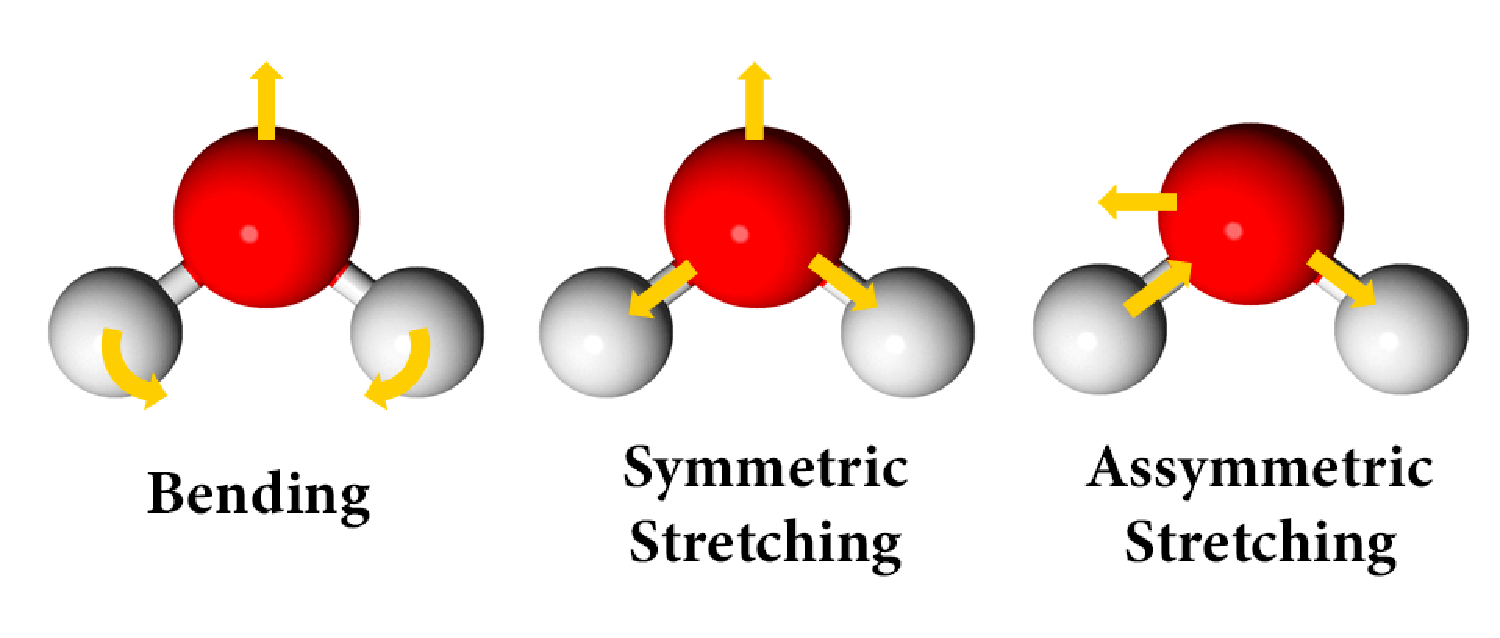
\includegraphics[scale=0.32]{figs/setas.pdf}
	\legend{Fonte: Compilação da autora.}
\end{figure}
 
\begin{table}[b!]
 	\centering
 	\caption{Tabela contendo as frequências ($ \si{cm}^{-1} $) dos modos normais do monômero isolado, computacional e experimental, e das moléculas adsorvidas no Pd em diferentes orientações. \label{tab:modos}}
 	\begin{threeparttable}
 		\begin{tabular}{ccccccccc} 
 			\hline\hline\addlinespace[3.6pt]
 			\multicolumn{9}{c}{\textbf{Frequências dos Modos Normais (\si{\cm}$ ^{-1} $) - Monômero}}                                                                                                                            \\ 
 			\midrule
 			\multirow{3}{*}{}              & \multicolumn{2}{c}{Bending}              &  & \multicolumn{2}{c}{\textit{Stretching} (S)}                &  & \multicolumn{2}{c}{\textit{Stretching} (AS)}               \\ 
 			\cmidrule{2-3}\cmidrule{5-6}\cmidrule{8-9}&PBE & VDW-BH &  & PBE &VDW-BH&  & PBE &VDW-BH \\ 
 			\midrule Flat   & 1621& 1606             &  & 3651              &3599             &  &3741            & 3694              \\ 
 			Up & 1641& 1645  &  & 3768              & 3719              &  & 3879              & 3842               \\		
 			Down & 1590             &
 			1562           &  & 3624              & 3565   &  & 3694              & 3637               \\				 H$ _2$O Isolado  & 1672             &1665
 			&  & 3692             &  3641  &  & 3791             &   3745           \\ \midrule
 			H$ _2 $O Isolado Exp.\tnote{$\dagger$} & \multicolumn{2}{c}{1596.9}                         &  & \multicolumn{2}{c}{3632.5}                   &  & \multicolumn{2}{c}{3725.7}                       \\ \hline\hline
 		\end{tabular}
 		\begin{tablenotes}\footnotesize
 			\item[$\dagger$] \citeauthor{ref-modos}
 		\end{tablenotes}
 	\end{threeparttable}
 	\legend{Fonte: compilação da autora.}
 \end{table}
 
 Dessa forma, com o intuito de analisar as alterações nas propriedades vibracionais que a adsorção no metal provoca nos modos normais de um monômero, calculamos as frequências de vibração para cada orientação e em seguida comparamos aos valores experimentais e teóricos do monômero isolado (Tabela \ref{tab:modos}).
 
 As frequências obtidas via simulações computacionais com o funcional VDW-BH para o monômero isolado foram as que mais se aproximaram dos valores experimentais obtidos por meio de espectroscopia de infravermelho \cite{ref-modos}. Para o modo de vibração \textit{bending} as vibrações diferem entre $ 4\% $ e $ 5\%$ do valor experimental para os funcionais VDW-BH e PBE, respectivamente; em relação às frequências de \textit{stretching} simétrico e antisimétrico as variações são 1.6 e $1.8\% $ para o funcional PBE e 0.2 e $0.5\% $ para o funcional VDW-BH, respectivamente. 

 Para as estruturas adsorvidas foi usado como parâmetro de comparação os valores do monômero isolado obtido via simulações. Assim, para o modo \textit{bending} observa-se a maior diminuição (deslocamento para o vermelho - \textit{redshift}) para a orientação \textit{down}, $ \delta_{PBE}\sim 80 \,\si{\cm}^{-1}$ e $ \delta_{VDW-BH}\sim 100 \,\si{cm}^{-1}$. As configurações \textit{up} tiveram os menores \textit{redshift} na frequência de \textit{bending}: entre $ 20 $ e $ 30 \,\si{cm}^{-1}$ para os funcionais PBE e VDW-BH, respectivamente.

Em relação às frequências de \textit{stretching}, houve um aumento entre $ \sim 80 \,\si{cm}^{-1}$ e $ \sim 100 \,\si{cm}^{-1}$ nas frequências da orientação \textit{up}. Esse aumento decorre do fato de que nessa orientação não há interação entre os átomos de hidrogênio e a superfície metálica, logo essas frequências descrevem uma molécula mais covalente e com ligações O-H mais fortes. Por outro lado, os menores valores de frequências correspondem às estruturas \textit{down} com diminuições entre $ \sim 80 \,\si{cm}^{-1}$ e $ \sim 110 \,\si{cm}^{-1}$. Isso ocorre devido à interação da molécula com a superfície metálica e indica uma interação mais intensa. Para a molécula \textit{flat} as diminuições nas frequências foram entre $40$ e $ 60 \,\si{cm}^{-1} $. Esse comportamento de \textit{redshift} revela como a adsorção no metal modifica significativamente a ligação covalente O-H da molécula de água. 

 Por fim, comparando os valores obtidos entre o funcional PBE e VDW-BH, observa-se que o funcional VDW-BH fornece valores menores, particularmente para os modos de \textit{stretching}. Assim, com o funcional VDW-BH as moléculas de água se tornam menos covalentes e se ligam mais fortemente ao metal, fazendo com que as frequências de \textit{stretching} diminuam \cite{adrien}.  
%Modos Normais - Monômero 

Nessa seção revisitamos o problema da adsorção do monômero em superfícies metálica com o intuito de caracterizar a interface água metal, uma vez que esse problema motivou diversas investigações teóricas e experimentais ao longo dos últimos anos \cite{salmeron,monomerexp1, monomerexp2,michaedelis,monomer,adrien,review_new}. Do ponto de vista experimental, a adsorção da água em vários metais foi estudada utilizando-se especialmente Microscopia de Tunelamento com Varredura (\textit{Scanning tunneling microscopy} - STM) \cite{salmeron,monomerexp1,monomerexp2}. Todavia, essas caracterizações são dificultadas pela tendência das moléculas de água de se agruparem em clusters e pelo fato de que técnicas de STM não são suficientemente sensíveis para revelar a estrutura interna de moléculas adsorvidas \cite{michaedelis}. Por outro lado, no âmbito da eletrostática a orientação que favorece a interação com o metal é a molécula perpendicular à superfície \cite{adrien}. Nessa perspectiva, o uso de simulações computacionais permitiu esclarecer tais questões ao revelar que a molécula adsorve paralelamente e diretamente acima do átomo metálico (sítio \textit{atop}).

Assim, nossos resultados corroboram com os achados da literatura e mostram que a estrutura \textit{flat} é a mais estável seguida da orientação \textit{up}. Além disso, os resultados revelaram que o funcional VDW-BH intensifica a ligação da molécula de água com o metal. Como resultado, as energias de adsorção aumentam e as frequências de \textit{stretching} diminuem. Em relação às características estruturais do sistema, temos que a célula unitária de tamanho $ 6\times4\times4 $ descreve melhor a geometria do sistema, uma vez que diminui interações fictícias, ao passo que a convergência da energia é atingida com $ 2\times2 $ pontos k. Por fim, através de análises da estrutura eletrônica e de caracterizações estruturais e vibracionais, vimos como a adsorção no metal afeta a molécula de água. Essas caracterizações serão complementadas no capítulo seguinte ao investigar como essas propriedades são alteradas pela aplicação de um potencial externo. Além disso, na seção seguinte completaremos a caracterização da interface água/metal ao analisar como as ligações de hidrogênio são afetadas pela presença da superfície metálica através da adsorção de uma camada de água. No capítulo \ref{cap:bias}

\section{Camada de Água adsorvida no Pd(111)\label{sec:re-la}}
\subsection*{Propriedades estruturais e eletrônicas}
Após caracterizar as interações e as propriedades geométricas e vibracionais do monômero adsorvido, essas análises foram estendidas para camadas de água bidimensionais de tamanhos $ (\sqrt{3}\times\sqrt{3})R30\si{\degree} $ (\textit{bilayers}) adsorvidas sobre uma superfície metálica de Pd. A estrutura dessa camada é similar aos planos (0001) e (111) do gelo \textit{bulk}, no qual cada molécula de água forma 3 ligações de hidrogênio e estão arranjadas em hexágonos de tamanhos proporcionais ao parâmetro de rede do metal. Nesse modelo, metade das moléculas de água estão na orientação \textit{flat} e diretamente ligadas ao metal, além de atuarem como doadoras em ligações de hidrogênio com as moléculas adjacentes. A outra metade das moléculas não está diretamente ligada ao metal e forma três ligações de hidrogênio com as moléculas adjacentes - duas ligações atuando como receptor e uma como doador. Assim, as moléculas com orientações \textit{flat} estão em distâncias $ d_{OM} $ diferentes das demais moléculas. Esses modelos foram baseados em resultados experimentais de STM, nos quais foram observadas estruturas de clusters de água hexagonais em diversos metais, em especial no Pd(111) (Figura \ref{fig:layer_stm})  \cite{layer_dft,review,review2,review_new}

\begin{figure}[H]
	\centering
	\caption{(a) Imagens de clusters de $ D_2O $ adsorvidos no Pd(111) a 100K obtidas via STM ($ 175\times135\,\si{\angstrom} $); (b) ampliação de $ 41\times53\,\si{\angstrom} $ e (c) ampliação $ 20\times20\,\si{\angstrom} $.}
	\includegraphics[scale=0.7]{figs/layer_stm.png}
	\legend{Fonte: \citeauthor{layer_dft}}
	\label{fig:layer_stm}
\end{figure}  

A partir dos arranjos hexagonais observados nos experimentos de STM os modelos de camada bidimensional propostos sugerem que metade das moléculas estejam nas configurações \textit{flat} e as demais nas configurações \textit{flat-down} (camada \textit{H-down}) ou nas orientações \textit{flat-up} (camada \textit{H-up}) -- representadas na Figura \ref{fig:complete}. Além disso, os modelos consideram que as camadas podem ser formadas por uma mistura das orientações descritas acima (Fig. \ref{fig:complete}c) ou também apresentar moléculas dissociadas \cite{layer_dft}. Assim, nessa seção analisamos o efeito da adsorção no metal nas ligações de hidrogênio através das propriedades das camadas \textit{H-down}, \textit{H-Up} e \textit{H-Down/Up}.

\begin{figure}[b!]
	\centering
	\caption{Representação das três camadas de água do tipo bilayer utilizadas nas simulações computacionais. }
	\includegraphics[scale=0.3]{figs/complete2.png}
	\legend{Fonte: Compilação da autora.}
	\label{fig:complete}
\end{figure}  

Para descrever as camadas utilizamos células unitárias com 16 moléculas de água adsorvidas sobre uma superfície de Pd de tamanho $ 6\times4\times4 $. Escolhemos esse tamanho de superfície pois, de acordo com os resultados do monômero, essa superfície apresentou melhores resultados. Além disso, considerando a convergência do monômero adsorvido a partir de $2\times2$ pontos k, calculamos as energias de adsorção das camadas de acordo com os esquemas de pontos k: $1\times1$ e $2\times2$. Durante a otimização os átomos metálicos eram mantidos fixos e as moléculas de água eram relaxadas. Para cada esquema calculamos a energia considerando também correção dos erros de superposição de bases (BSSE). Os funcionais de troca e correlação utilizados foram PBE e VDW-BH.

As propriedades geométricas analisadas foram obtidas a partir da média sobre as distâncias entre os átomos de oxigênio (${d_{OO}}$), entre os átomos de oxigênio e de paládio (${d_{OM}}$) e entre os átomos de hidrogênio e oxigênio (${d_{OH_1}}$ e ${d_{OH_2}}$) para cada uma das moléculas que compõem as camadas e suas respectivas orientações \textit{flat}, \textit{flat-down} e \textit{flat-up} (Figura \ref{fig:geometric}). Em relação à definição de qual átomo de hidrogênio corresponde a $H_1$ ou $H_2$, adotou-se a convenção de que nas orientações \textit{flat-up} e \textit{down} o átomo que faz ligação de hidrogênio é $H_1$ e o que está ``livre'' é denominada $H_2$. 


\begin{figure}[H]
	\centering
	\caption{Distâncias interatômicas analisadas na camada de água adsorvida no Pd.} 
	\includegraphics[scale=0.43]{figs/geometric.png}
	\legend{Fonte: Compilação da autora.}
	\label{fig:geometric}
\end{figure}

 
Diferentemente do monômero adsorvido, a definição da energia de adsorção da camada não é tão direta. Isso ocorre pela dificuldade em separar as diferentes contribuições para a energia. Assim, adotando as definições apresentadas por \citeauthor{adrien}, a energia de adsorção da camada ($ E_{ads} $) é definida como a energia média por molécula de água:
\begin{equation}
	E^{bilayer}_{ads}=-\frac{1}{n}\pqty{E_{all}-E^{bilayer}_{H_2O}- E_{metal}}
\end{equation}
onde $ n $ é o número de moléculas de água na célula unitária, $ E_{all} $ é a energia do sistema com a camada adsorvida, $ E_{metal} $ e $ E^{bilayer}_{H_2O} $ são as energias da superfície metálica e da camada de água calculados com a configuração atômica da camada, respectivamente. Essa energia representa o ganho de energia ao mover a camada de água do infinito à superfície de Pd.

Outra definição apresentada na literatura \cite{adrien} é a de energia de coesão, que corresponde à energia necessária para criar uma camada bidimensional de gelo acima da superfície de Pd(111):

\begin{equation}\label{eq:coesao}
	E_{coesão/H_2O}=\frac{1}{n}\pqty{E_{all}-n\cdot E_{isolated}-E_{metal}}
\end{equation}
onde nesse caso, $E_{isolated}$ é a energia de um monômero isolado, multiplicado pelo número de moléculas $n$. Normalmente, os resultados reportados na literatura \cite{adrien,layer} correspondem à energia de coesão.

%DOADOR É O $H_2$.

Como foi dito anteriormente, quando aumentamos a complexidade do sistema e passamos de um monômero adsorvido para uma camada aumentamos também a complexidade das interações. Nesse sentido, para analisar o efeito da adsorção no metal sobre as ligações de hidrogênio, faremos a comparação das propriedades analisadas com as do dímero no vácuo. Isso se dá pelo fato de esse sistema é um protótipo da ligação de hidrogênio, logo a comparação das propriedades da camada de água adsorvida em relação às do dímero no vácuo revela o efeito do metal sobre as ligações de hidrogênio e detalhes a interação água/metal \cite{monomer}.
\begin{table}[b!]
	\centering
	\caption{Tabela com as energia de ligação (eV) e as distâncias entre os átomos de oxigênio $d_{OO}$ ($\si{\angstrom}$) e entre os átomos de hidrogênio e oxigênio $d_{OH}$ ($\si{\angstrom}$) do dímero de água no vácuo calculadas com os funcionais PBE e VDW-BH, bem como o valor experimental. Nos dois casos, o valor $d_{OH}=0.98\,\si{\angstrom}$ correspondem à ligação O-H doadora na ligação de hidrogênio. \label{tab:dimero}}
	\begin{threeparttable}
		\begin{tabular}{ccccccc} 
			\hline\hline
			\multicolumn{7}{c}{ \textbf{Dímero no Vácuo} }        \\ \midrule
			&  & Energia ($ \si{\eV} $)                                  &  & $ d_{OO}(\si{\angstrom})$                                         &  & $ d_{OH}(\si{\angstrom})$                \\\midrule
			PBE    &  & 0.26                                   &  & 2.90                                         &  & 0.97/0.98                              \\
			VDW-BH &  & 0.24                                   &  & 2.91                                         &  & 0.97/0.98                              \\
			Exp.\tnote{$\dagger$}   &  & 0.23                                   &  & 2.98                                         &  &  -                                      \\
			\hline\hline
		\end{tabular}
		\begin{tablenotes}\footnotesize
			\item[$\dagger$] \citeauthor{dimer-exp}
		\end{tablenotes}
	\end{threeparttable}
\end{table}
\begin{table}[t!]
	\centering
	\caption{Propriedades geométricas das camadas de água H-Down, H-Up e H-Down/Up. Após os átomos atingirem as posições de mínimo, foi medido para cada camada a distância média entre os átomos de oxigênio ($ {d_{OO}} $). Considerando as diversas orientações das moléculas que compões as camadas, foi medido para cada tipo de orientação a distância média entre o átomo de O e de Pd ($ {d_{OM}} $) e as distâncias médias entre o oxigênio e os átomos de hidrogênio ($ {d_{OH_1}}$ e $ {d_{OH_2}}$).\label{tab:camada}}
	\begin{tabular}{cccccccccccc} 
		\hline\hline\addlinespace[3.5pt]
		\multicolumn{12}{c}{\textbf{Propriedades Geométricas ($ \si{\angstrom} $) - Camada de Água}}                                                                                                                                                                                                              \\ 
		\midrule
		\multicolumn{3}{c}{\multirow{2}{*}{\textbf{Camada}}}                                                                                                  &  & \multicolumn{2}{c}{\textbf{H-Down}} &  & \multicolumn{2}{c}{\textbf{H-Up}} &  & \multicolumn{2}{c}{\textbf{H-Down/Up}}  \\ 
		\cmidrule{5-6}\cmidrule{8-9}\cmidrule{11-12}
		\multicolumn{3}{c}{}                                                                                                                                  &  & PBE  & VDW                      &  & PBE  & VDW                     &  & PBE  & VDW                             \\ 
		\midrule
		&                                                                                       & ${d_{OO}}$   &  & 2.84 & 2.81                         &  & 2.86 & 2.83                       &  & 2.87 & 2.83                               \\ 
		\midrule
		\multirow{9}{*}{\textit{Moléculas}} & \multirow{3}{*}{\textit{Flat}}                                                        & ${d_{OM}} $ &  & 2.66 & 2.50                         &  & 2.68 & 2.52                       &  & 2.59 & 2.46                               \\
		&                                                                                       & ${d_{OH_1}}$ &  & 0.99 & 1.00                         &  & 0.99 & 0.99                       &  & 0.99 & 0.99                               \\
		&                                                                                       & ${d_{OH_2}}$  &  & 0.99 & 1.00                         &  & 0.99 & 0.99                       &  & 0.99 & 0.99                               \\ 
		\cmidrule{2-12}
		& \multirow{3}{*}{\begin{tabular}[c]{@{}c@{}}\textit{Flat}\\\textit{Down}\end{tabular}} & ${d_{OM}} $ &  & 3.06 & 2.99                         &  & -    & -                          &  & 3.05 & 2.99                               \\
		&                                                                                       & ${d_{OH_1}}$  &  & 0.99& 1.00                         &  & -    & -                          &  & 0.99 & 1.00                               \\ 
		&                                                                                       & ${d_{OH_2}}$  &  & 1.00 & 1.01                         &  & -    & -                          &  & 1.00 & 1.02                               \\
		\cmidrule{2-12}
		& \multirow{3}{*}{\begin{tabular}[c]{@{}c@{}}\textit{Flat}\\\textit{Up}\end{tabular}}   & ${d_{OM}} $ &  & -    & -                            &  & 3.20 & 3.08                       &  & 3.29 & 3.15                               \\
		&                                                                                       & ${d_{OH_1}}$ &  & -    & -                            &  & 1.00 & 1.00                      &  & 1.00 & 1.00                               \\
		&                                                                                       & ${d_{OH_2}}$ &  & -    & -                            &  & 0.97 & 0.97                       &  & 0.97 & 0.97                               \\
		\hline\hline
	\end{tabular}	
	\legend{Fonte: compilação da autora.}
\end{table}

Para tanto, iniciamos os cálculos eletrônicos com dímero no vácuo e analisamos as distâncias entre os átomos de Oxigênio ($d_{OO}$) e a a energia de ligação -- Tabela \ref{tab:dimero}. O funcional VDW-BH forneceu a energia (0.24 eV) mais próxima ao experimental (0.23 eV) e as distâncias $ d_{OO} $ estão de acordo com o experimental \cite{dimer-exp}. Considerando a camada de água adsorvida no metal (Tabela \ref{tab:camada}), observa-se que as distâncias $ d_{OO} $ diminuem em relação ao dímero no vácuo devido à presença do metal. Em especial, essa redução é maior para os resultados obtidos com o funcional VDW-BH nas três camadas, $2.81\;\AA$ e $2.83\;\AA$ comparados com $2.91\;\AA$ do dímero no vácuo. Além disso, observa-se que a camada H-Down apresenta as menores distâncias $d_{OO}$, portanto, do ponto de vista estrutural essa camada possui a ligação de hidrogênio mais intensa e mais estável. Portanto, a adsorção no metal diminui as distâncias entre as moléculas e intensifica as ligações de hidrogênio, visto que quanto mais forte a ligação de hidrogênio, menor é a distância $d_{OO}$. 

O efeito da presença do metal sobre as ligações de hidrogênio é refletido nas demais medidas, tais como a distância $d_{OM}$. Comparando o valor $ d_{OM} $ das moléculas \textit{flat} da camada de água com o monômero \textit{flat} adsorvido no metal, observa-se um aumento médio de $ 0.25\,\si{\angstrom} $ para o funcional PBE e $ 0.17\,\si{\angstrom} $ para o funcional VDW-BH. Além disso, para as moléculas \textit{flat} da camada de água, observa-se uma discrepância de $ 0.15\,\si{\angstrom} $ entre os funcionas, com as menores distâncias pertencendo ao funcional VDW-BH. Os resultados obtidos via PBE para as distâncias $d_{OM}$ estão de acordo com o trabalho realizado por \citeauthor{adrien}, ao passo que, os resultados que obtivemos com o funcional VDW-BH estão cerca de $ 0.2\,\si{\angstrom} $ menores que os reportados para o funcional VDW-DRSLL para as moléculas da camada \textit{H-Down} e $ 0.4\,\si{\angstrom} $ para as moléculas da camada \textit{H-Up}.
%Dímero





%Propriedades Geométricas PBE - Layer
\begin{table}[b!]
	\centering
	\caption{Energia de adsorção de cada camada de água, de acordo com cada funcional, quantidade de pontos k e com a presença ou não de BSSE.\label{tab:agua}}
	\begin{tabular}{cccccccccc} 
		\hline\hline
		\multicolumn{10}{c}{\textbf{Energias de Adsorção - Camada de Água (eV})}                                                                                           \\ 
		\midrule
		&   \multicolumn{4}{c}{PBE}                                      &      &  \multicolumn{4}{c}{VDW-BH}                                             \\ 
		\cmidrule{1-10}
		\textit{Pontos k} &   \multicolumn{2}{c}{$1\times1$} &  \multicolumn{2}{c}{$2\times2$} & & \multicolumn{2}{c}{$1\times1$} &  \multicolumn{2}{c}{$2\times2$}  \\ 
		\cmidrule{1-10}
		\textit{Correção} & - & BSSE                 & - & BSSE                   &    & - & BSSE                  & - & BSSE                       \\ 
		\midrule
		H-Down            & 0.20 & 0.12                  & 0.18 & 0.10                     & & 0.58 & 0.30                   & 0.37 & 0.28                   \\
		H-Up             & 0.12 & 0.05                   & 0.11 & 0.04                &      & 0.47 & 0.20                    & 0.27 & 0.19                     \\
		H-Down/Up    & 0.17 & 0.10                  & 0.16 & 0.08                  &   & 0.54 & 0.26               & 0.33 & 0.24                     \\
		\hline\hline
	\end{tabular}
	\legend{Fonte: Compilação da autora.}
\end{table}
\begin{table}[b!]
	\centering
	\caption{Energia de coesão de cada camada de água comparado com os valores encontrados na literatura para cada funcional. O valor registrado corresponde à camada com $2\times2$ pontos k e com correção BSSE.\label{tab:coesao}}
	\begin{threeparttable}
		\begin{tabular}{ccccccccc} 
			\hline\hline
			\multicolumn{9}{c}{\textbf{Energias de Coesão - Camada de Água (eV})}       \\ 
			\midrule
			&  & \multicolumn{3}{c}{PBE} &  & \multicolumn{3}{c}{VDW-BH}  \\ 
			\cmidrule{3-5}\cmidrule{7-9}
			&  & Eq.\eqref{eq:coesao}  &  & Ref.\tnote{*}       &  & Eq.\eqref{eq:coesao}  &  & DRSLL\tnote{*}    \\ 
			\midrule
			H-Down         &  & 0.58 &  & 0.47        &  & 0.72 &  & 0.42           \\
			H-Up           &  & 0.54 &  & 0.40          &  & 0.68 &  & 0.42           \\
			H-Down/ Up &  & 0.58 &  & -             &  & 0.72 &  & -              \\
			\hline\hline
		\end{tabular}
		\begin{tablenotes}\footnotesize
			\item[*] \citeauthor{adrien}
		\end{tablenotes}
	\end{threeparttable}
	\legend{Fonte: compilação da autora.}
\end{table}


Seguindo a convenção adotada em relação ao átomo H referente às distâncias ${d_{OH_1}}$ e ${d_{OH_2}}$, percebemos um aumento das distâncias comparadas com o dímero no vácuo, com exceção dos valores $ d_{OH2} $ das moléculas \textit{flat-up}. Além disso, as distâncias ${d_{OH_2}}$ das moléculas na orientação  \textit{flat-down} são maiores que ${d_{OH_1}}$, ou seja, as ligações água/metal alargam a distância $d_{OH}$ mais que as ligações de hidrogênio. Isso ocorre para os dois tipos de camada que incluem essa orientação e as distâncias $ d_{OH2} $ diferem em até $ 0.04\,\si{\angstrom} $ em relação ao dímero isolado,. Para as moléculas na orientação \textit{flat-up}, apenas as ligaçoes O-H que participam da ligação de hidrogênio ${d_{OH_1}}$ são afetada e apresentam um aumento de $ 0.02\,\si{\angstrom} $ em relação à ligação O-H do dímero que participa da ligação de hidrogênio; ao passo que, para a distância ${d_{OH_2}}$, onde o átomo H que está ``livre'' não ocorre nenhuma modificação. Isso é observado nas camadas H-Up e na H-Down/Up. Em relação às moléculas \textit{flat}, todos os comprimentos ${d_{OH}}$ são alongados, uma vez que todas essas moléculas participam de uma ligação de hidrogênio. % Além disso, esse resultado indica que a interação da molécula com o metal é mais forte que a ligação de hidrogênio. 

%\todo[inline,color=green!40]{Falta falar sobre os gráficos de densidade de carga.}

Em relação à energia de adsorção do sistema (Tabela \ref{tab:agua}), vemos que a presença da correção de erros de superposição de bases melhora o valor da energia. Para o funcional PBE, a utilização da correção BSSE diminui a energia entre 0.07 e 0.08 eV em relação aos valores sem correção. Ademais, para o funcioal PBE o aumento de pontos k não influencia a energia, com variações de 0.01 e 0.02 eV. Entretanto, para o funcional VDW-BH o aumento da quantidade de pontos k provoca uma diminuição de $ 0.21\,\si{\eV}$ para o caso sem correção. Além disso, com o funcional VDW-BH, a correção BSSE faz com que as energias se aproximem e independa da quantidade de pontos k. Portanto, erros de superposição afetam o valor da energia, pois, ao utilizar a correção BSSE os valores das energias se aproximam e a quantidade de pontos k não afeta a convergência.
%Energia de Adsorção

Além da energia de adsorção, calculamos também a energia de coesão (Tabela \ref{tab:coesao}) com $2\times2$ pontos k e correção BSSE para cada funcional e comparamos com os valores reportados na literatura \cite{adrien}. Os resultados que obtivemos para o PBE divergem em cerca de $ 0.13\,\si{\eV} $ dos valores relatados por \citeauthor{adrien}. Essa divergência pode estar relacionada ao número de moléculas utilizadas na célula unitária para descrever a camada, visto que no presente trabalho utilizamos 16 moléculas em comparação a 2 moléculas utilizadas pelos autores. Para o funcional VDW-BH, o nosso valor foi superior ao obtido pelos autores com o funcional VDW-DRSLL. Além disso, nesse trabalho os autores relataram que de acordo com os resultados obtidos não houveram diferenças energéticas, e em relação as camadas H-Down e H-Up os valores que obtivemos mostram que isso ocorre entre as camadas H-Down e H-Down/Up. A partir da análise estrutural e energética, observamos que a camada H-Down e H-Down/Up são as estruturas mais estáveis para os dois tipos de funcional. Isso ocorre devido à interação água/metal que é maior nas moléculas de orientação \textit{flat-down}. Além disso, os cálculos com o funcional VDW-BH forneceram energias maiores que o PBE. 

%energia de coesão


Após calcular as energias de adsorção, obtemos os gráficos de diferenças de densidade de carga para cada camada além da densidade média ao longo do eixo z (Figura \ref{fig:densidade_layer}). Através dos gráficos, vemos que a interação das moléculas \textit{flat} com a camada ocorrem através da interação do orbital $ b_1$ com o orbitais \textit{d} do metal, assim como foi visto no monômero. Também observamos um aumento da densidade de carga na região ao redor dessas moléculas. Esse aumento é mais intenso na região entre as moléculas \textit{flat-down} e o metal. Ademais, observa-se que as interações com o metal ocorrem principalmente pelas moléculas \textit{flat} e \textit{flat-down}, de modo que as moléculas \textit{flat-up} praticamente não interagem com o metal. 


\begin{figure}[H]
	\centering
	\caption{(a) Diferenças de densidades de carga $\Delta\rho$ das camadas H-Down, H-Up e H-Down/Up na superfície de tamanho $6\times4\times4$ e calculadas com os funcionais PBE e VDW-BH. Para todos os casos, o valor da isosuperfície foi $1.20 \times10^{-3}\;e/\AA$, onde vermelho (azul) indica uma diminuição (aumento) da densidade de carga durante a adsorção. (b)  $ \Delta\rho $ médio ao longo do eixo z de acordo com as camadas para os funcionais PBE(lado esquerdo) e VDW-BH(lado direito). As linhas tracejadas correspondem às posições dos átomos da última camada metálica de Pd e às posições dos átomos O e H das moléculas \textit{flat-down} e \textit{flat-up} nas respectivas camadas. \label{fig:densidade_layer}}
	\begin{subfigure}{0.45\textwidth}            
		\caption{\textit{Diferença de Densidade de Carga} ($ \Delta\rho $)}
		\centering
		\includegraphics[width=\textwidth]{figs/z_charge.png}
		\legend{Fonte: compilação da autora}
		\label{fig:camada_dens}
	\end{subfigure}
	\begin{subfigure}{0.8\textwidth}
		\caption{\textit{Diferença de Densidade de Carga Média ao longo do eixo z.}}
		\centering
		\includegraphics[width=\textwidth]{figs/pd_camada_z.png}
		\legend{Fonte: compilação da autora.}
		\label{fig:camada_z}
	\end{subfigure}
\end{figure}


Através do gráfico de diferença de carga média ao longo do eixo z (Figura \ref{fig:camada_z}), observa-se que as os valores de $ \Delta\rho $ foram maiores com o funcional VDW-BH. Para a camada H-Down, observa-se que o efeito das moléculas \textit{flat-down} sobre $ \Delta\rho $ é mais intenso. Em particular, na região entre a molécula \textit{flat-down} e o metal nota-se uma diminuição acentuada no valor de $ \Delta \rho $. Por outro lado, as modificações que ocorrem na camada \textit{H-Up} são exclusivamente devido à molécula \textit{flat}, visto que as moléculas \textit{flat-up} não interagem diretamente com o metal. A camada H-Down/Up preserva as características das duas outras camadas, porém a interação da molécula \textit{flat-down} é menos intensa. Para compreender melhor como essas interações afetam a estrutura intramolecular das moléculas de água investigaremos na próxima seção os modos normais de vibrações. 


\subsection*{Modos normais de vibração}

Com o intuito de corroborar e completar as análises estruturais e energéticas realizadas e analisar o efeito da adsorção no metal sobre as ligações de hidrogênio, calculamos para cada estrutura as frequências de vibrações dos modos normais. Isso possibilitou identificar as frequências relacionadas à cada tipo de interação (água-água e água-metal). Para representar as frequências do sistema, utilizamos uma distribuição normalizada, uma vez que nosso sistema é composto por 16 moléculas e a quantidade de modos normais de vibrações são dados por $ 3\times N-6 $. Assim, na Figura \ref{fig:modos} está a distribuição para cada funcional, bem como as frequências do dímero isolado experimental (linha pontilhada). Na Tabela \ref{tab:modos}, representamos os valores inferiores e superiores das frequências de \textit{stretching} e o valor central da frequência de \textit{bending}.

Através dessas frequências podemos obter informações sobre a intensidade da ligação de hidrogênio e sobre as interações água/metal, uma vez que é possível relacionar as frequências com as respectivas interações. Essas análises são feitas comparando os valores da camada adsorvida com os valores do dímero no vácuo e explorando as modificações provocadas pelo metal. Por exemplo, uma alta frequência do modo de \textit{stretching} indica uma fraca ligação O-H e também uma ligação de hidrogênio menos intensa e vice-versa. Assim, através dos modos normais de vibrações podemos analisar qual interação é mais dominante em cada estrutura \cite{ref-modos}.
%Modos Normais - Camada
\begin{table}[b!]
	\centering
	\caption{Tabela contendo as principais frequências de vibração da camada adsorvida de acordo com cada funcional, bem como as frequências experimentais e teóricas do dímero isolado. \label{tab:freq-camada}}
	\begin{threeparttable}
		\begin{tabular}{cccccccccc} 
			\hline\hline\addlinespace[3.6pt]
			\multicolumn{10}{c}{\textbf{Frequências dos Modos Normais (cm$ ^{-1} $) - Camada de Água}}                                                                                                                                         \\ 
			\midrule
			\multirow{3}{*}{}                                                &  & \multicolumn{2}{c}{\multirow{2}{*}{Bending}} &  & \multicolumn{5}{c}{\textit{Stretching} (S)}                                                                                                                          \\
			&  & \multicolumn{2}{c}{}                         &  & \multicolumn{2}{c}{Inferior}                                               &  & \multicolumn{2}{c}{Superior}                                                \\ 
			\cmidrule{3-4}\cmidrule{6-10}
			&  & PBE  & VDW                                &  & PBE  & VDW                                                                 &  & PBE  & VDW                                                                 \\ 
			\midrule
			H-Down                                                         &  & 1695 & 1683                                  &  & 3193 & 3051                                                                &  & 3500 & 3428                                                                 \\ 
			
			H-Up                                                           &  & 1664 & 1642                                  &  & 3292 & 3228                                                                &  & 3823 & 3777                                                                 \\ 
			
			H-Down/ Up                                                 &  & 1682 & 1664                                  &  & 3101 & 3180                                                                &  & 3803 & 3774                                                                 \\\midrule  Dímero Isolado            &  & 1668 & 1661                                 &  & \begin{tabular}[c]{@{}c@{}}3612\\3857\end{tabular} & \begin{tabular}[c]{@{}c@{}}3605\\3841\end{tabular}                                                                &  & \begin{tabular}[c]{@{}c@{}}3776\\3875\end{tabular} & \begin{tabular}[c]{@{}c@{}}3752\\3850\end{tabular}                                                                 \\ 
			\midrule Dímero Isolado Exp.\tnote{$\dagger$} &  & \multicolumn{2}{c}{1618.1}                   &  & \multicolumn{2}{c}{\begin{tabular}[c]{@{}c@{}}3547.5\\ 3697.7\end{tabular}} &  & \multicolumn{2}{c}{\begin{tabular}[c]{@{}c@{}}3625.5\\3714.7\end{tabular}}  \\
			\hline\hline
		\end{tabular}
		\begin{tablenotes}\footnotesize
			\item[$\dagger$]\citeauthor{ref-modos}
		\end{tablenotes}
	\end{threeparttable}
	\legend{Fonte: compilação da autora.}
\end{table}




Em relação às frequências de \textit{stretching} do dímero isolado experimental, temos que as frequências $3547.5$ e $3697.7\,\si{cm}^{-1}$ correspondem às frequências de \textit{stretching} simétrico (S) e assimétrico (AS) da molécula doadora, respectivamente, de modo que o menor valor correspondente à ligação O-H que participa da ligação de hidrogênio; as frequências $3625.5$ e $3714.7\,\si{cm}^{-1}$ correspondem às frequências de \textit{stretching} S e AS molécula receptora. Comparando as frequências do dímero isolado obtidas com os funcionais PBE e VDW-BH em relação ao valor experimental, vemos que os valores estão superestimados em média $ 3.3\% $. 
\begin{figure}[t!]
	\centering
	\caption{Distribuição das frequências ($\si{cm}^{-1}$) de vibrações das camadas de acordo com o funcional utilizado. As linhas sólidas e tracejadas correspondem aos funcionais PBE e VDW-BH, respectivamente; as linhas pontilhadas são as frequências experimentais do dímero isolado.}
	\includegraphics[scale=0.4]{figs/graph_pbe.png}
	\legend{Fonte: compilação da autora.} 
	\label{fig:modos}
\end{figure}

Analisando as frequências da Tabela \ref{tab:modos}, vemos que \textit{bending} da camada H-Up é menor que o valor calculado para o dímero isolado, em especial para o funcional VDW-BH. Isso acontece porque nas moléculas \textit{flat-up} uma ligação O-H participa da ligação de hidrogênio e a outra não se liga ao metal, diferentemente das camadas H-Down e H-Down/Up. Portanto, a camada H-Up é a que possui a intensidade da ligação de hidrogênio mais fraca. Essa observação é também sustentada pelas frequências de \textit{stretching}, onde os maiores valores pertencem à camada H-Up. Por outro lado, as frequências de \textit{stretching} da camada H-Down constituem os menores valores. Esse resultado mostra o efeito da interação com o metal nos modos normais de vibração. A camada H-Down/Up apresenta as propriedades semelhantes às outras duas, com a frequência de \textit{stretching} inferior próxima a da H-Down e a frequência \textit{stretching} superior próxima a H-Up. 

Quando tratamos da frequência de vibração do dímero, temos bem definido quais frequências pertencem às ligações O-H das moléculas doadoras e das receptoras. Entretanto, quando estudamos as camadas adsorvidas, temos além da ligação de hidrogênio a interação com o metal. Ou seja, temos as vibrações da ligação O-H das moléculas \textit{flat} que fazem ligação de hidrogênio e atuam como doadoras ou receptoras; as ligações O-H das  moléculas \textit{flat-up} e \textit{flat-down} que participam das ligações de hidrogênio como doadoras; além das ligaçoes O-H que interagem com o metal (\textit{flat-down}) ou que estão ``livres'' (\textit{flat-up}). 

Analisando a camada H-Down para ambos funcionais, temos 4 picos de frequências de \textit{stretching}, onde um está mais afastado dos demais. Através de uma animação realizada no Programa \textit{Jmol}\footnote{As animações estão disponíveis no link: \url{https://shre.ink/u5l}} é possível ver que, o primeiro pico corresponde à interação da molécula \textit{flat-down} com o metal; o seguinte corresponde à ligação O-H da molécula \textit{flat-down} que faz ligação de hidrogênio e os demais correspondem às moléculas \textit{flat}. Além disso, nota-se que todos os picos dessa camada estão abaixo das frequências do dímero experimental. Como frequências de \textit{stretching} mais baixas correspondem a intensidade das ligações de hidrogênio maiores, então a adsorção no metal fortalece a ligação de hidrogênio. 

Em relação a camada H-Up, o pico de maior frequência está relacionado à ligação O-H que não faz ligação com o metal e as demais estão relacionadas às ligações O-H que participam das ligações de hidrogênio. Por fim, como foi dito anteriormente, a camada H-Down/Up preserva as propriedades de ambas camadas, de modo que os primeiros picos correspondem às interações das moléculas \textit{flat-down} com o metal, o último refere-se às ligações O-H da molécula \textit{flat-up} que estão ``livres'' e os demais correspondem às interações água/água.


Por fim, após caracterizar a adsorção de camadas de água sobre o metal, vimos que o metal intensifica a ligação de hidrogênio entre as moléculas de água através da diminuição da distância $ d_{OO} $. Além disso, vimos que a camada H-Down é mais estável energeticamente e provoca uma diminuição de densidade de carga na região entre a molécula \textit{flat-down} e o metal. Por outro lado, a presença de moléculas \textit{flat-down} na camada H-Down/Up também a torna estável, uma vez que essa camada preserva as características da camada H-Down. Através das propriedades vibracionais, vimos que a interação com o metal apresenta frequências de \textit{stretching} menores que as frequências correspondentes às ligações de hidrogênio. Nesse capítulo caracterizamos a interface água/metal sem a presença de uma pertubação externa ao sistema. No próximo capítulo analisaremos se as caracterizações aqui realizadas são afetadas pela presença de um potencial externo.
